\chapter{METODE PENELITIAN}

Bab ini memaparkan tentang metodologi penelitian yang digunakan pada penelitian ini.

\section{Analisis penyelesaian masalah}

Pada permasalahan pencarian Ulam non-interaktif, penjawab tidak diperbolehkan menjawab sebelum penanya selesai menanyakan seluruh query. Pendekatan pertama yang mungkin untuk menyelesaikan permasalahan ini adalah dengan mempersiapkan pencarian biner. Namun pencarian biner tidak dapat menyelesaikan masalah kebohongan dalam jawaban. Oleh karena itu diperlukan pendekatan statistik peluang menggunakan pembobotan berlekamp. Gambar \ref{fig:flow_berlekamp} menjelaskan alur proses adalah membuat query pencarian biner terlebih dahulu, lalu dioptimasi menggunakan fungsi pembobotan berlekamp untuk menghitung peluang dari semua angka-angka dalam range $S_n$.

\begin{figure}
\centering
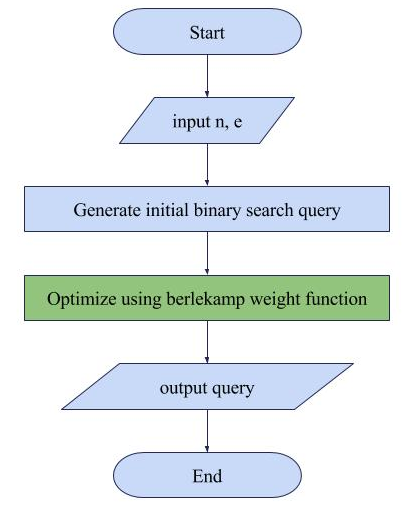
\includegraphics[scale=0.4]{../img/flowchart-berlekamp.png}
\caption{Diagram alir solusi menggunakan pembobotan Berlekamp}
\label{fig:flow_berlekamp}
\end{figure}

\begin{figure}
\centering
\begin{BVerbatim}
1001101
0101011
0010111
\end{BVerbatim}
\caption{Generator matrix $[7,3,4]_2$}
\label{fig:generator734}
\end{figure}

\begin{figure}
\centering
\begin{BVerbatim}
0000000  1000111
0011101  1000111
0101011  1000111
0110110  1000111
\end{BVerbatim}
\caption{Perfect binary code $(7,8,4)_2$}
\label{fig:binarycode784}
\end{figure}

Now again see a generator matrix $[7,3,4]_2$ in Figure \ref{fig:generator734} can create a perfect binary code $(7,8,4)_2$ code in Figure \ref{fig:binarycode784}. A generator matrix $[n, m, d]_2$ where $n = 2^m - 1$ and each \textbf{column} is a linear combination of $m$ bit binary string except $\vec{0}$ can make a perfect binary code $(n,M,d)_2$ where $d = M/2$. \textbf{\textit{We need a profing or citation..}}

Nah masalahnya, jika $d$ yang kita butuhkan kurang dari $M/2$, maka kita harus menggunakan seminimal mungkin $n$ kolom pertama $[M-1,M,M/2]_2$ sehingga menghasilkan $[n,M,d]_2$. Asumsikan kita memiliki fungsi $\aleph(d)$ adalah berapa kolom pada generator matrix yang akan menghasilkan kode biner dengan minimal jarak Hamming $d$. Hal yang pasti adalah $\aleph(M/2) = M-1$ dan $\aleph(1) = {log}_2(m)$ (need proving). Worst case adalah $\aleph(d)=M/2 + d - 1$. Best case adalah karena ada $M-1$ kolom untuk $0 \leq d \leq M/2$, maka $\aleph(d) = d/2$ (sepertinya tidak mungkin). Nah problem kita adalah bagaimana mengurutkan kolom pada generator matrix sehingga $\aleph(d)$ sesempurna mungkin, atau bisa dikatakan $\aleph(d) - \aleph(d-1) \approx 2$.
